\chapter{UCNA Analysis}
\label{ch:UCNA_Analysis}
%%%%%%%%%%%%%%%%%%%%%%%%%%%%%%%%%%%%%%%%%%%%%%%%%%%%%%%%%%%%%%%%%%%%%%%%%%%%%%%
%%%%%%%%%%%%%%%%%%%%%%%%%%%%%%%%%%%%%%%%%%%%%%%%%%%%%%%%%%%%%%%%%%%%%%%%%%%%%%%
%%%%%%%%%%%%%%%%%%%%%%%%%%%%%%%%%%%%%%%%%%%%%%%%%%%%%%%%%%%%%%%%%%%%%%%%%%%%%%%

\iffalse
Designing an experiment and collecting the right data are non-trivial alone,
but interpreting the results lends itself to a whole new train of thought.
The rest of this thesis is spent describing the details of such an
analysis, with this chapter summarizing important aspects,
such as terminology to be used later and the
model used to characterize our detector response.
\fi

This chapter is dedicated to introducing important aspects of the analysis that
are not strictly tied to calibrations and asymmetry extraction, but rather to the
data collection and processing required to turn raw detector signals into values that
can be calibrated and analyzed. 





%--------------------------------------------------------------

\section{Outline of Analysis Steps} \label{sec:outline}

To preface the rest of this chapter, we begin by highlighting
the general process of the analysis beginning with a raw detector
ADC value from each PMT and finishing with an asymmetry.
Below are the general steps for processing the data:

\begin{itemize}
\item Determine pedestals for each PMT and subtract the pedestal from each data event.
\item Measure the gain of each PMT and remove any time-dependent drifts from the signal.
\item Apply a PMT-by-PMT calibration to determine the expected position dependent
  energy deposited in the scintillator
  for each event.
\item Correct for the position dependent response of each PMT $i$
  to return a visible energy for each PMT, $E_{\mathrm{vis},i}$.
\item Combine the four PMT energies into a single deposited energy, $E_{\mathrm{vis}}$.
\item Convert this combined estimate of the energy deposition to a final
  reconstructed energy, $E_{\mathrm{recon}}$, to use in analysis.
\item Calculate an asymmetry and apply all systematic corrections.
\end{itemize}

Simulations of the experimental apparatus and particle transport are also intertwined
in the analysis. By simulating the underlying physical processes, we gain an understanding
as to what the signals in our detector indicate regarding the initial event. The simulations
consist of particle tracking and the summation of energy losses throughout
the spectrometer, and also a Detector Response Model to transform the simulation variables
into detector-like signals. This process will be addressed in Section \ref{sec:DetectorResponseModel}.

It is important to point out early on the difference between $E_{\mathrm{vis}}$ and
$E_{\mathrm{recon}}$. The  visible energy, $E_{\mathrm{vis}}$, is an estimate of the energy
physically deposited in the
scintillator by a particle, while the reconstructed energy, $E_{\mathrm{recon}}$, is an estimate of
the true initial energy of an event. The two are different due to the electron losing energy
as it traverses through the windows of the decay trap, the windows of the MWPC,
the MWPC itself, and the dead layer of the scintillator. These energy losses are not
``visible'' as the energy loss is not captured by any active detector component\footnote{The MWPC is technically
  an active detector, but it is not used as part of the energy calibration of the electron, and thus losses in
the wirechamber decrease the energy visible in the scintillator.}.
Of course the analysis could be
done in terms of $E_{\mathrm{vis}}$, but it is more convenient to express the results
in terms of the true electron energy spectrum, and also the energy dependent theory modifications
are in terms of the true initial energy of the $\beta$-decay electrons.

The majority of the analysis described throughout this thesis was completed using
the ROOT Data Analysis Framework \cite{brun1997root}. A special thanks goes out to
the Nuclear and Particle Physics communities as a whole, who have collectively built an indispensible
web of documentation regarding any and all things ROOT. Without the ROOT documentation
and user community, much of this analysis would have been painstakingly more difficult.




\section{Time-dependent Detector Corrections}

Obviously the system is not immune to drifts in signals due to variations
in time. There are many sources of such drifts, ranging from simple
electronic noise to changes in temperature. We deal with time-dependent
effects using pedestal subtraction, gain correction, and constant monitoring
of backgrounds.

\subsection{Pedestal Subtraction} \label{ssec:pedSubtraction}
The pedestal is a measure of the underlying detector signal, or baseline, 
upon which all other data signals lie. In terms of PMT signals, you can imagine 
the pedestal as a non-zero ADC value corresponding to zero input, or an offset.
You might say that the experiment can be run without caring about an offset
because the calibration will take this into account, which would be the case 
if the pedestals were constant or if we calibrated each run against itself, but 
neither is the case. We use a collection of consecutive runs to form our 
calibration sets, and these sets then calibrate data which is often taken hours,
or even days, earlier or later. Thus time-dependent pedestals can be worrisome, and care
must be taken to determine the pedestals and subtract them from data signals.

To determine a pedestal, events must be chosen where there was a global trigger, but
the PMT of interest does not trigger and preferably there is no signal
whatsoever in the scintillator on that side. Obvious choices for these events are
UCN monitor triggers, opposite side two-fold PMT triggers, and high-threshold $^{207}\mathrm{Bi}$
pulser triggers from other PMTs. Once there is a global trigger, we can use the individual TDC
to ensure there was no individual trigger, and the events can be 
histogrammed for the PMT of interest. The mean of the pedestal
peak can be taken as the average pedestal for a single run,
and this value can be 
subtracted from every subsequent reading of this PMT.

\begin{figure}[p]
\centering
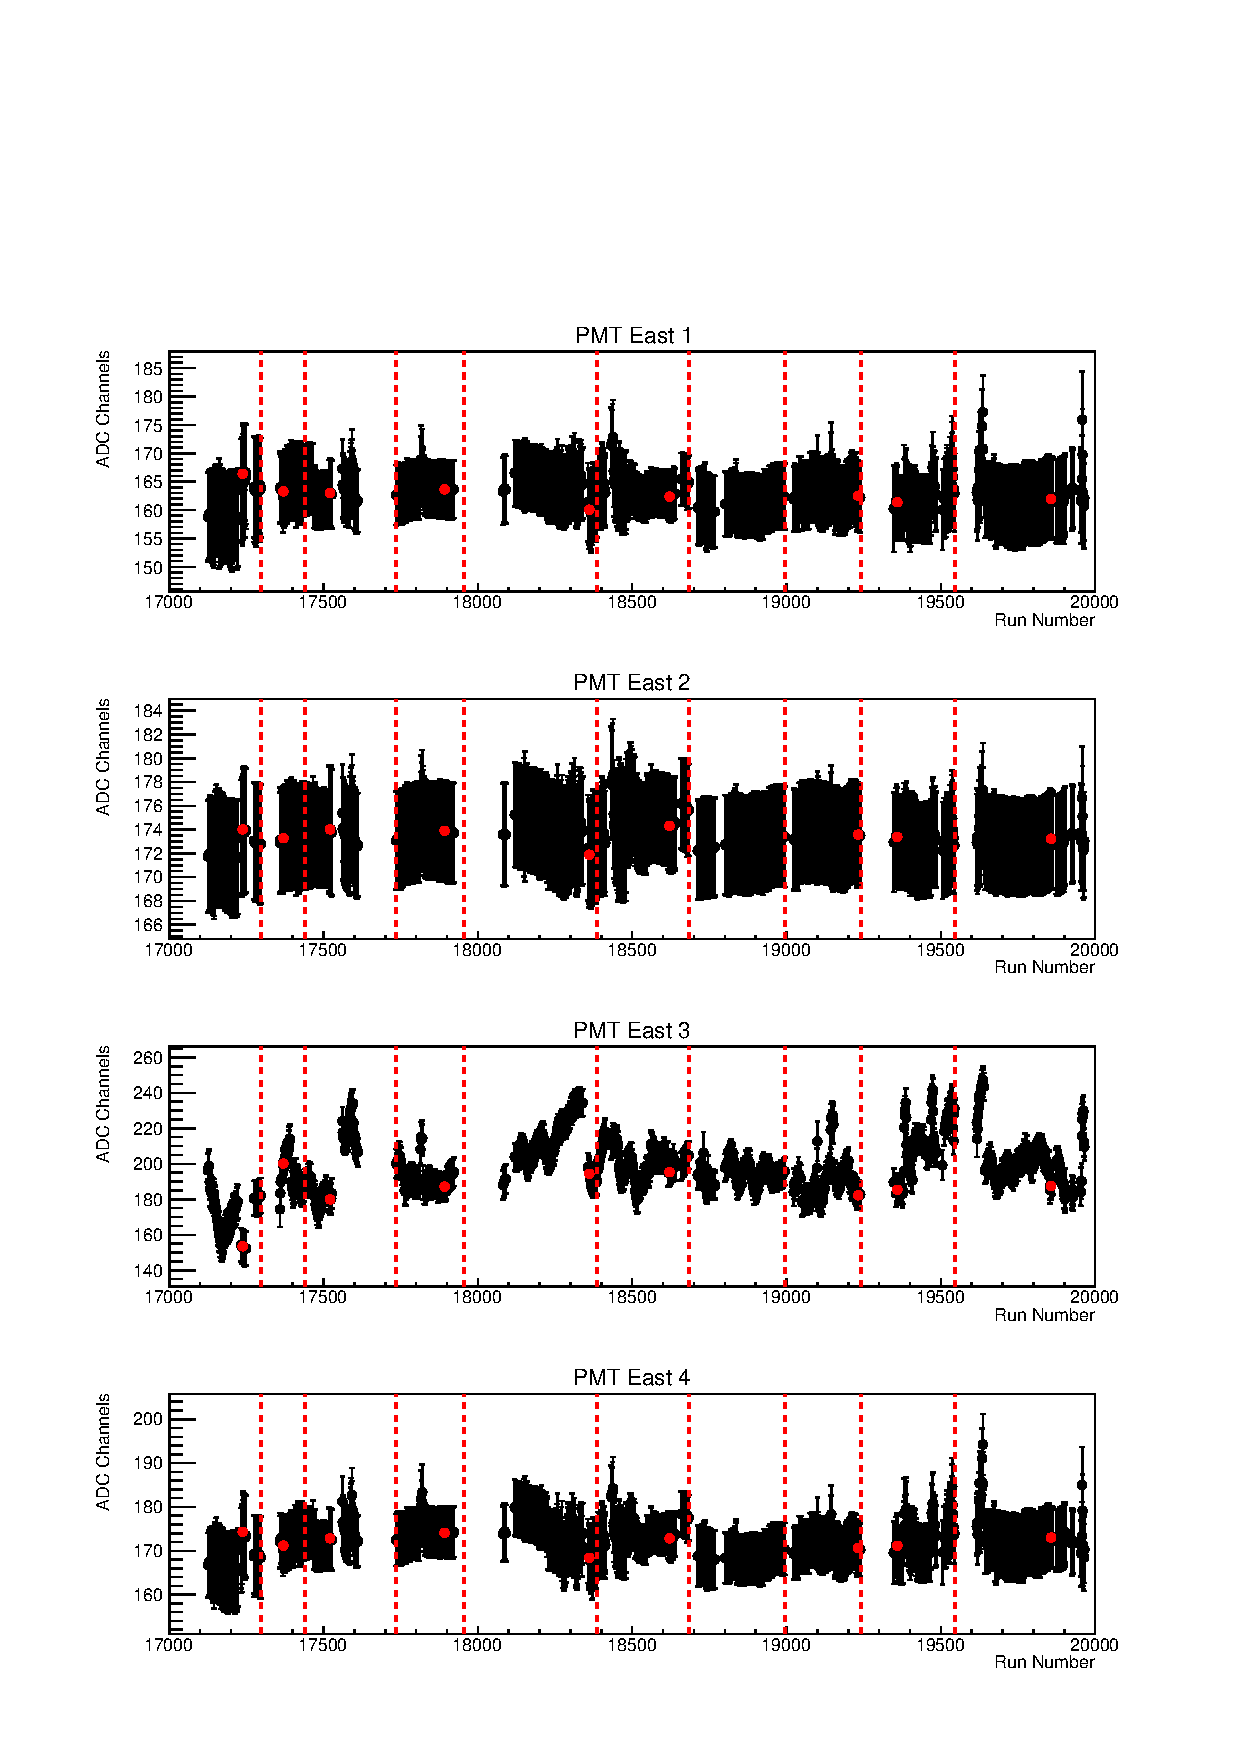
\includegraphics[page=1,scale=0.8]{3-UCNAAnalysis/2011-2012_pedestals.pdf}
\caption{Pedestal means as a function of run number for 2011-2012 East Detectors. Error bars are the
  RMS of the measured pedestal. The red lines indicate what ranges of runs belong to
  different calibration periods, and the red marker is the calibration reference run,
  which will be discussed in later sections. Missing periods of data indicate some sort of failure
  from that PMT, and so it was removed from the analysis over that period.}
 \label{fig:peds_timeDep}
\end{figure}

\begin{figure}[p] 
\centering
\includegraphics[page=2,scale=0.8]{3-UCNAAnalysis/2011-2012_pedestals.pdf}
\caption{Pedestal means as a function of run number for 2011-2012 West Detectors. Error bars are the
  RMS of the measured pedestal. The red lines indicate what ranges of runs belong to
  different calibration periods, and the red marker is the calibration reference run,
  which will be discussed in later sections. Missing periods of data indicate some sort of failure
  from that PMT, and so it was removed from the analysis over that period.}
\label{fig:peds_timeDep}
\end{figure}

One interesting thing to note is that the discriminators, which determine whether
a component triggers,
for all PMTs are housed 
together, which leads to correlations between the PMT triggers. In a perfect world, 
each PMT would have one pedestal, and that pedestal wouldn't care about other PMT's signals.
Instead, what we see is that the pedestals
can be dependent on the type of events that are chosen 
to construct the pedestal, and the effect can be $\sim10$~channels for some PMTs.
This indicates that the pedestal for one PMT may be dependent
on the signal present in another PMT. These shifts are important as a
pedestal shift of 5-10 channels maps to an offset of roughly
5-10 keV, as the PMTs show close to 1:1 correspondence between ADC and keV.

The influence of event type on pedestal values means we must carefully choose which events
to use when calculating the pedestal.
The best choice would be UCN monitor events due to there being zero signal 
in the electronics box housing the PMT electronics, and these thus would give
the cleanest measurement of the PMT pedestal.
These are unfortunately the first event type we can eliminate as they are only present
during $\beta$-decay runs (when UCN are produced and thus create UCN monitor triggers)
and not during calibration runs (taken during the day when the beam is off). 
Of the remaining two options, the choice was made to use the
two-fold PMT triggers from the opposite detector rather than $^{207}\mathrm{Bi}$ pulser
events. The choice is somewhat arbitrary, because what is important is that we choose
a consistent subset of data for both calibration and $\beta$-decay data, but the
opposite side two-fold triggers do better represent the baseline present in each PMT
for data events when compared to the much higher signal present from the $^{207}\mathrm{Bi}$
pulser.


\iffalse
\begin{figure}[h] 
\centering

\includegraphics[scale=.25]{3-UCNAAnalysis/ImageHolder.pdf}
\caption{Pedestal values for a $\beta$-decay run determined using different 
types of events to illustrate the cross-talk between PMTs. (UCN Monitors, 
Bi triggers, Opposite side triggers, same side 2-fold triggers. Also shown 
is the dependence of the pedestal on which PMT triggers in the Bi Pulser. NOTE:
Choose West PMT4 in an early 2012/2013 beta run) }
\label{fig:peds_types}
\end{figure}

\begin{figure}[h] 
\centering

\includegraphics[scale=.25]{3-UCNAAnalysis/ImageHolder.pdf}
\caption{Example pedestals from all 8 PMTs}
\label{fig:peds_ind}
\end{figure}
\fi



With the event type chosen, we extract the mean and RMS of the pedestal peak
for each PMT in every run. The pedestal mean (referred to as simply
the pedestal) is then subtracted from the ADC values for all events. This effectively
removes the time-dependent baseline from the detector signals. The time dependence of
the pedestals can be seen for the East PMTs from 2011-2012 in Figure \ref{fig:peds_timeDep}.
Most of the PMTs have pedestals which remain quite stable, but PMT East 3 shows the
importance of a run-by-run pedestal subtraction.



\subsection{Gain Correction} \label{ssec:BiGain}

\subsubsection{$^{207}\mathrm{Bi}$ Pulser}
%The goal of the $^{207}\mathrm{Bi}$ gain monitoring pulser system is to create a standard
%candle type signal present in all PMTs to be tracked over time. 
The primary gain monitoring system consists of a small amount of $^{207}\mathrm{Bi}$
deposited within a small block of scintillator. The scintillator was surrounded by
light reflecting material on three sides, with the fourth side covered with an optical
attenuator to attempt to match the light output of the $\sim$1~MeV conversion line in the $^{207}\mathrm{Bi}$
to the light output of 1~MeV of energy deposited in the detector scintillator. The pulser was then
attached directly to the PMT next to where the light guides attached to the PMT.
To allow for a single-PMT high threshold trigger, the signal was split off to a different
discriminator than the one used when determining a two-fold trigger. These high threshold
discriminators then allowed for pulser triggers with a distinct pulser identification \cite{mpmThesis}.

An unfortunate but low impact issue with the pulser involves the amount of attenuation applied to the
pulser signal. The pulser peak lies well beyond the equivalent of 1~MeV of light as would be produced
in the detector scintillator, and therefore far outside the range of the $\beta$-decay spectrum.
For the level of precision achieved with this experimental configuration, this
is not a limiting issue as the PMTs seem to be quite linear, so even a peak well outside the
energy range of interest should suffice.

\begin{figure}[h] 
\centering
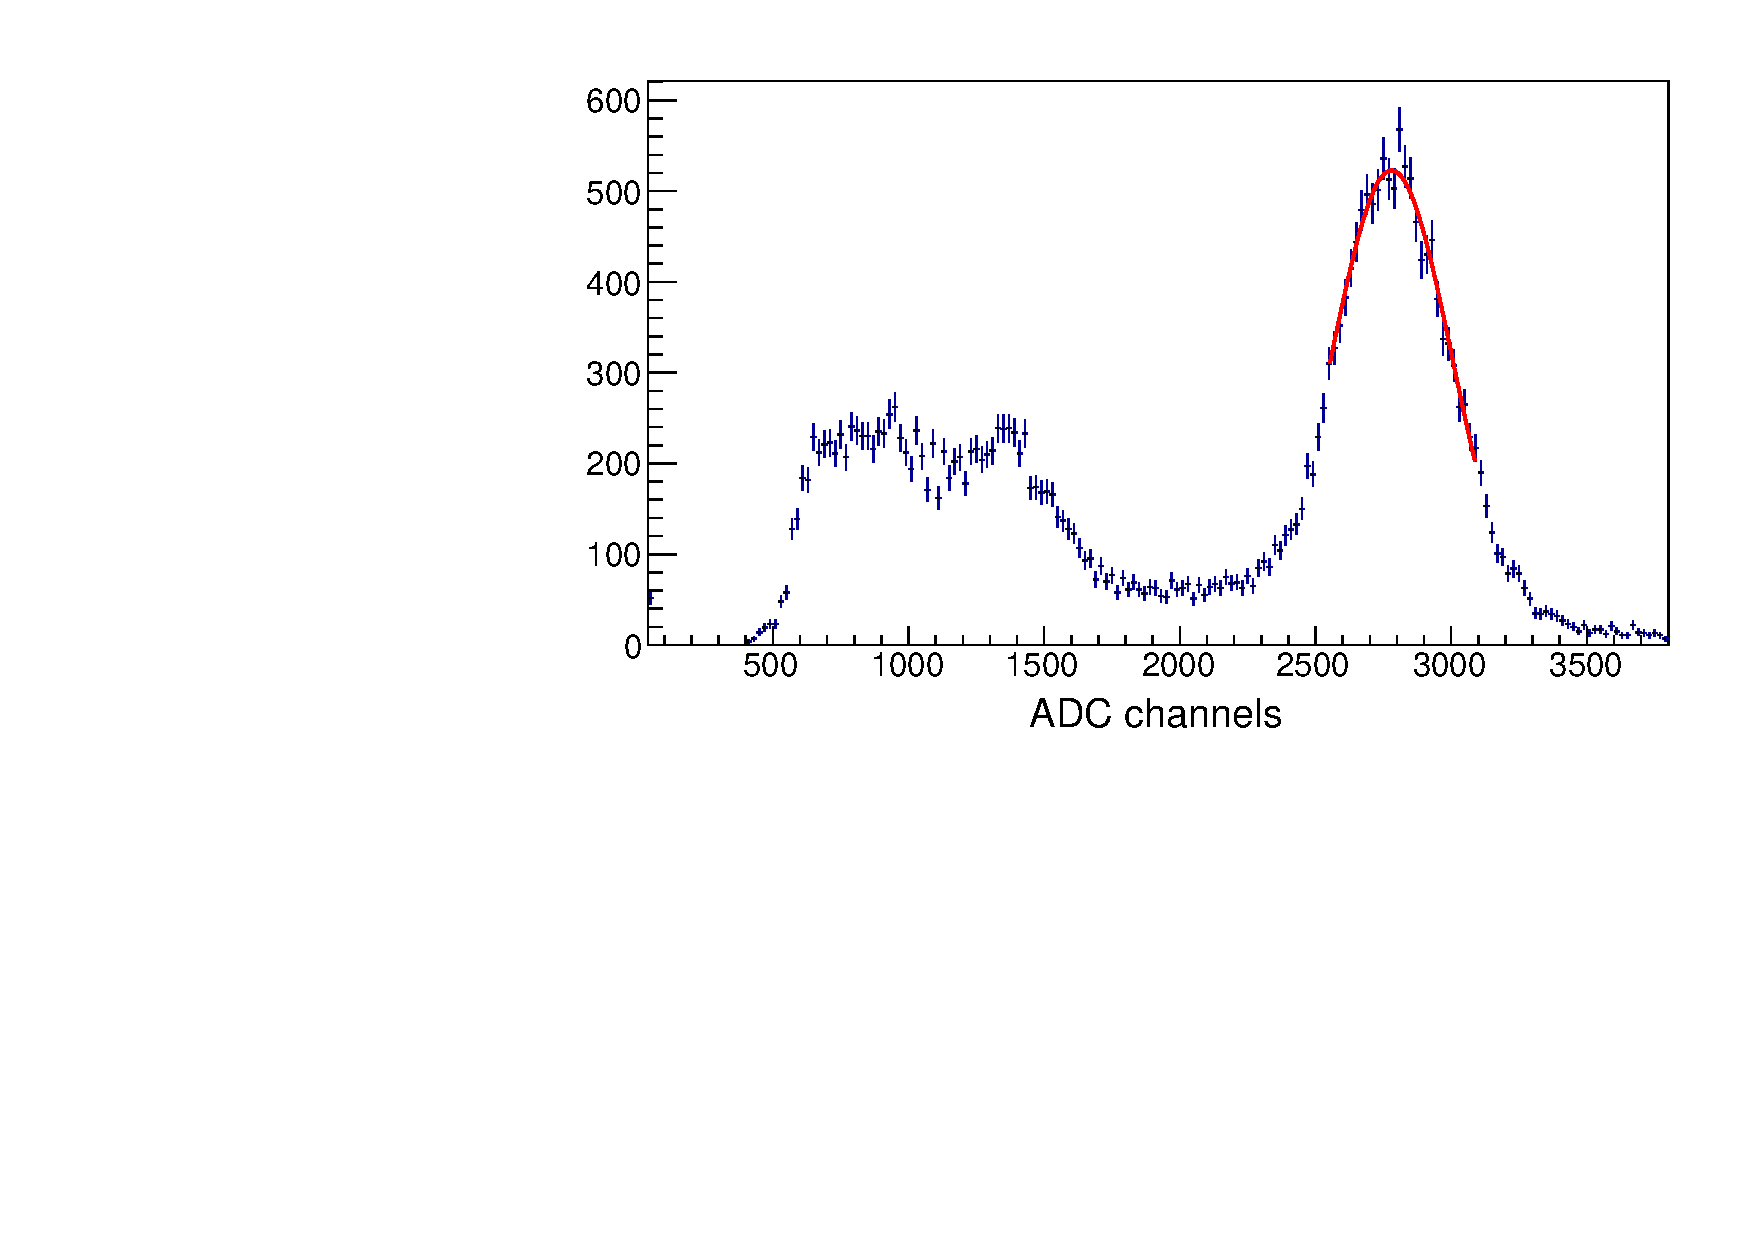
\includegraphics[scale=.60]{3-UCNAAnalysis/gain_bismuth2.pdf}
\caption{Example $^{207}\mathrm{Bi}$ spectrum and fit for a single PMT over
  the course of a run. The upper and lower bismuth conversion electron peaks are
  seen, along with a distribution from the compton scattering of decay gammas. Note that the gamma rays are
  visible because the pulser is attached directly to the PMT and there is no type
  of veto (like the MWPC) to remove them.}
\label{fig:biPulser}
\end{figure}

The $^{207}\mathrm{Bi}$ pulser peak is fit by a Gaussian on a run-by-run basis, allowing for gain corrections on the time
scale of a single run. The fit was done iteratively, with the initial guesses for mean and fit range determined
by stepping backwards from the last bin and using a self-written algorithm to search for the peak. Then the peak
was fit five times consecutively, with each successive fit being fed the previous fit's mean and sigma. This
made sure the fit converged as best as possible on the mean of the pulser peak. An example pulser peak and fit
can be seen in Figure \ref{fig:biPulser}. The asymmetric fit (range extends farther above the peak than below)
is actually a characteristic part of the iterative
fitting algorithm developed for use throughout this analysis. For Gaussian like peaks occurring as a result of
a process like energy loss in a scintillator followed by PMT amplification, the upper end of the peak is
inherently more Gaussian due to the lower end having a tail from extraneous energy losses. 

The method for applying the gain correction is as follows. First, a reference gain must be determined
to normalize all other gains against. This was chosen to be what is called the ``reference run'', and it
typically consists of a manually inspected source run within each source calibration period. The gain factor
is then calculated as the ratio of the pulser peak in a given run divided by the pulser peak in the reference
run, or
%
\begin{equation}
  g_i = \frac{\mu_i}{\mu_{\mathrm{ref}}}
\end{equation}
%
This automatically defines the gain of the reference run to be $g_{\mathrm{ref}}=1$. Then all other runs which are
calibrated by a certain run period have gain factors which vary based on the fitted pulser value. The time
dependence of the gain values in 2011-2012 can be seen in Figures \ref{fig:2011-2012pulser_East}
and \ref{fig:2011-2012pulser_West}. The behavior is similar in 2012-2013.

Some problems with the $^{207}\mathrm{Bi}$ pulser did occur. There were several periods where the pulser
simply did not work for a certain PMT. This was always limited to a single PMT not working at a given time, and when this
was the case the PMT without a pulser signal was not used when reconstructing the energy. This has
minimal effect on the energy reconstruction though, as the ``bad'' PMT is still used when determining
a two-fold trigger, and the remaining three PMTs contain sufficient information for reconstructing the
energy deposited. Periods where $^{207}\mathrm{Bi}$ pulser information is missing are evident in
Figure \ref{fig:2011-2012pulser_West} where there is missing data for certain PMTs over extended ranges.
It should be noted that in 2012-2013, West PMT4 never had a functioning pulser and was consequently never used for
energy reconstruction purposes.

\begin{figure}[p] 
  \centering
  \includegraphics[page=3,scale=.8]{3-UCNAAnalysis/2011-2012_gain.pdf}
  \caption{Gain factors, $g_i$, as a function of run number for 2011-2012 East Detectors.
    The red lines indicate what ranges of runs belong to
    different calibration periods, and the red marker is the calibration reference run.}
  \label{fig:2011-2012pulser_East}
\end{figure}

\begin{figure}[p] 
  \centering
  \includegraphics[page=4,scale=.8]{3-UCNAAnalysis/2011-2012_gain.pdf}
  \caption{Gain factors, $g_i$, as a function of run number for 2011-2012 West Detectors.
    The red lines indicate what ranges of runs belong to
    different calibration periods, and the red marker is the calibration reference run.}
  \label{fig:2011-2012pulser_West}
\end{figure}

\subsubsection{Endpoint Stabilization} \label{sssec:endpoint}

There are unexplained longer term gain fluctuations that do not seem to be captured by the
$^{207}\mathrm{Bi}$ gain monitoring system that can be seen by monitoring the endpoint of the
$\beta$-decay spectrum. These are corrected by applying a second gain factor, $g_{\mathrm{ep},i}$ for PMT $i$,
as the last step in the calibration process. This endpoint gain factor is determined
by comparing the endpoints as seen by each
calibrated PMT to the expected endpoint from the simulation. The final energy for each PMT
is then multiplied by this factor. This does not force the final reconstructed energy endpoint to
match the final reconstructed simulation endpoint exactly,
as the final spectra are the weighted average of the four PMT responses, but rather it corrects 
some systematically shifted periods of data which consistently exhibited endpoints $>30$~keV
away from the expected endpoint.

The method for calculating $g_{\mathrm{ep}}$ was developed previously by M. Mendenhall in section
5.2.2 of \cite{mpmThesis}. For the sake of clarity, the process is repeated here.

\begin{figure}
  \centering
  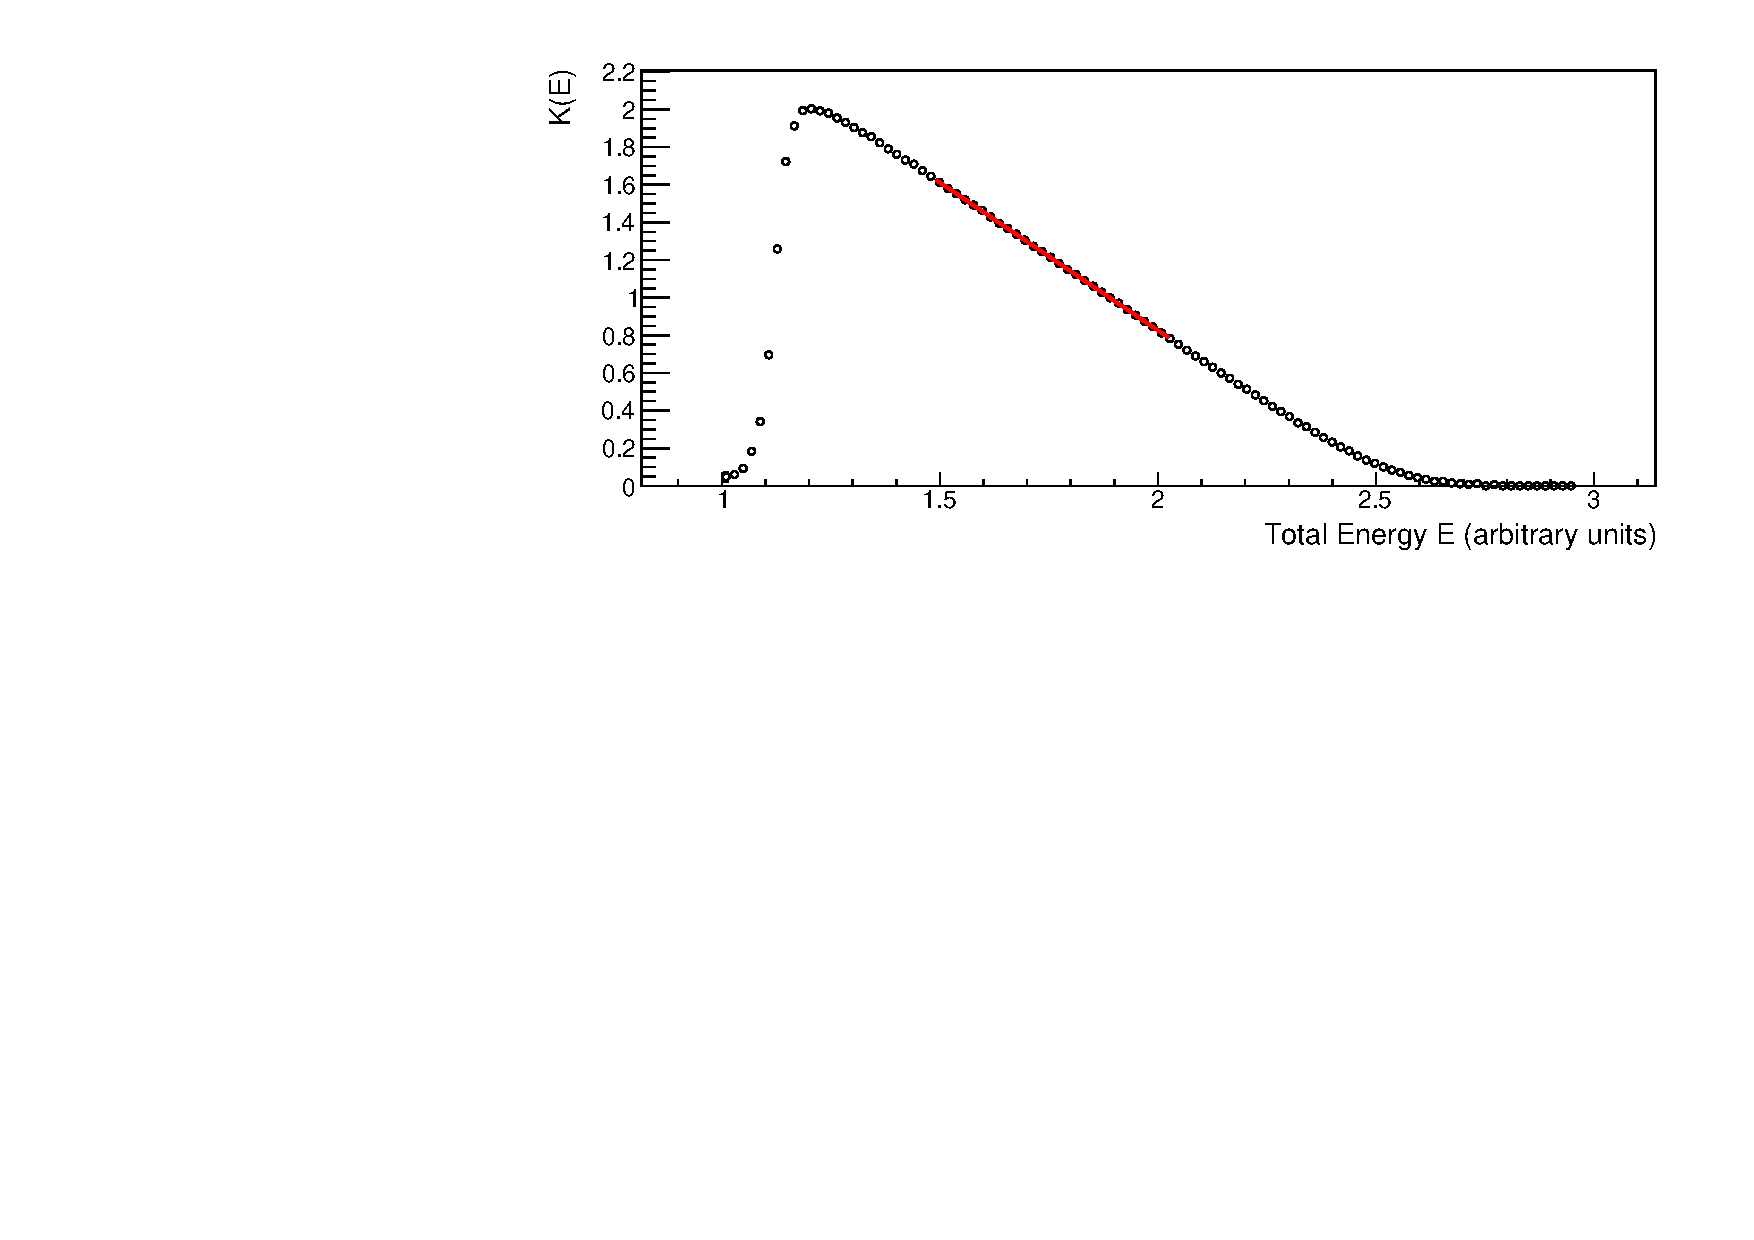
\includegraphics[scale=0.75]{3-UCNAAnalysis/kuriePlot.pdf}
  \caption{Example Kurie plot with linear fit to extract the y-intercept, which is
    the endpoint energy. The deviations from a straight line are due to the
    trigger efficiency at low energies and finite resolution at high energies. Care
    must be taken to fit in a region which most appropriately characterizes the true
    underlying electron energy spectrum.}
  \label{fig:kuriePlot}
\end{figure}
  

The endpoints are fit using a Kurie plot \cite{kurie1936radiations}, which linearizes the
energy response making for easy determination of the endpoint energy. If we approximate
the decay rate as the phase space factor for the neutron, then we can write down
the decay rate as a function of the electron total energy $E$, endpoint
energy $E_0$, and momentum $p$ as
%
\begin{equation}
  S(E) = pE\big(E_0-E\big)^2
\end{equation}
%
From this we see that a linear equation (the Kurie plot) can be formed:
%
\begin{equation}
  K(E) = \sqrt{\frac{S(E)}{pE}} = E_0-E
\end{equation}
%
where the $y$-intercept and $x$-intercept both determine the endpoint energy $E_0$.
An example Kurie plot can be seen in Figure \ref{fig:kuriePlot}.

Now we assume that the measured kinetic energy spectrum $T_{\mathrm{meas}}$ is different from the expected
kinetic energy spectrum $T_{\mathrm{sim}}$ by the gain factor $g_{\mathrm{ep}}$ such that
%
\begin{equation}
  T_{\mathrm{sim}} = g_{\mathrm{ep}} T_{\mathrm{meas}}.
\end{equation}
Then we can write the
measured total energy as
\begin{equation}
  E_{\mathrm{meas}} = m_e + g_{\mathrm{ep}}T_{\mathrm{meas}} \quad (c=1).
\end{equation}
The extracted endpoint for the data is now a function of $g_{\mathrm{ep}}$
since
\begin{equation}
  K(E_{\mathrm{meas}}) = \sqrt{\frac{S(E_{\mathrm{meas}})}{pE_{\mathrm{meas}}}} = E_{0,\mathrm{meas}}-E_{\mathrm{meas}},
\end{equation}
and upon proper choice of $g_{\mathrm{ep}}$, $E_{\mathrm{meas}}=E_{\mathrm{sim}}$. To solve for
the proper gain factor, the data endpoint is iteratively fit with the gain factor adjusted upon each iteration
according to
%
\begin{equation}
  g'_{\mathrm{ep}} = \frac{ E_{0,\mathrm{meas}}- m_e}{ E_{0,\mathrm{sim}}- m_e}g_{\mathrm{ep}} =  \frac{ T_{0,\mathrm{meas}}}{ T_{0,\mathrm{sim}}}g_{\mathrm{ep}}, 
\end{equation}
%
where $E_{0,\mathrm{meas}}$ is the extracted endpoint energy from the data with gain factor $g_{\mathrm{ep}}$ applied,
$E_{0,\mathrm{sim}}$ is the expected endpoint energy extracted from simulation, $T_0$ is the endpoint kinetic energy,
and $g'_{\mathrm{ep}}$ is the guess for the next iteration of endpoint fitting.
Once the condition $1-\frac{g'_{\mathrm{ep}}}{g_{\mathrm{ep}}}<10^{-7}$ is met, the value of $g'_{\mathrm{ep}}$ is taken as the final
endpoint gain factor and is saved to the calibration database. This process is carried out for each PMT for every
$\beta$-decay run, and then every event is reprocessed with the new gain factor applied to the visible energy from PMT
$i$ according to
%
\begin{equation}
  E_{\mathrm{vis},i}^{\mathrm{FINAL}} = g_{\mathrm{ep},i} E_{\mathrm{vis},i}.
\end{equation}
Then $E_{\mathrm{recon}}$ is calcuated using the final visible energies from the available PMTs.



\subsection{Time-Dependent Backgrounds}
Background events which may have some time dependence are removed from the analysis
via dedicated background runs that accompany every $\beta$-decay run.
Subtracting these background rates from the data rates accounts for backgrounds
with roughly a one hour time variation.
Any backgrounds that vary at the sub one hour level may go unnoticed, but
with a signal to background better than 50:1 the contribution from such is minimal.
Background subtraction will be addressed in Section \ref{sssec:bgsubtr}. 

\section{Trigger Thresholds} \label{sec:triggerThresh}

Looking ahead to the detector response model that will be implemented when processing
the simulated data, we need to determine the trigger thresholds for each of the
PMTs. With each PMT attached to a leading edge discriminator, the
amount of charge in a pulse that can create a trigger is randomized. The ADC signal
is an integrated signal, so two signals with integrated charge
at roughly the trigger threshold may have
different amplitudes and therefore different likelihoods of passing the discriminator threshold.
Measurement of these thresholds is important for the detector response model within the simulation
in order to properly model the low energy behavior of the measured spectrum.


\subsection{General Model for Trigger Determination} \label{ssec:genTrigModel}

The most important part of determining the trigger threshold shape for 
any detector is the availability of data which was collected no matter if 
the detector produced a trigger. If such a subset of 
data is available and plentiful, it is straightforward to estimate
the trigger probability by binning the data in some unit proportional to 
energy (whether in energy or something like it is not important) and taking 
the bin-by-bin ratio of those events that triggered to all of the events in the 
sample. Plotting these ratios as a function of whatever energy-like metric was chosen
depicts how probable an event of some value is to create a trigger. The resulting
trigger probability distribution can then be fit to extract a trigger function, and then
these functions can be sampled within simulation to apply a model of the
true trigger threshold to the simulated signals.


\subsection{Trigger Data Selection}
As mentioned before, the data used for constructing trigger thresholds must not be 
biased towards triggering the PMT of interest. Thus that PMT must not be a mandatory 
component of the global trigger for that event, and care must be taken to choose only 
events which would trigger regardless of the behavior of the PMT of interest. One
other stipulation placed on these events is that they have an opportunity to 
deposit energy in a particular scintillator. The best choice of events that 
satisfy these conditions are those that have a two-fold trigger on the opposite side 
and then backscatter and those that trigger at least three PMTs on the side of 
interest, which guarantees that the scintillator would have triggered with or without 
the PMT of interest.	

\subsection{Determining the Trigger Probability}
One option for determining the trigger probability function (and probably the 
most straightforward) is to calculate the trigger probability for an entire detector as 
a whole as a function of the energy deposited by an event. What you get is a 
function that provides the probability that an event of energy $ E_i $ 
produces some sort of trigger in that 
detector. Initially this method was employed in this analysis for sake of simplicity, and it produced 
reasonable agreement between simulation and data, but there is one 
glaring concern: Determining this trigger function from data requires that the data be 
calibrated first. At first glance this may not seem like much of an issue, but the 
calibration hinges upon the 
simulated peaks at low energy, which in turn rely on the trigger functions. This 
cyclical dependence hinders one from truly understanding any discrepancy between 
simulation and data at low energies, which is exactly the reason this method was 
abandoned.  

Instead, similarly to previous analyses, we decided to calculate the trigger
function on a PMT-by-PMT basis as a function of ADC channels above pedestal. This
encompasses a true characteristic of each component of the detector rather than some
average effect as seen by a detector package, which is what the aforementioned 
method produces. A typical trigger threshold is seen in Figure \ref{fig:trigger_thresh}.
As illustrated in Section \ref{ssec:genTrigModel}, the ratio of triggering events
to all events was taken in each ADC bin and then fit using the method described
in the following section.
  

\begin{figure}[h] 
\centering
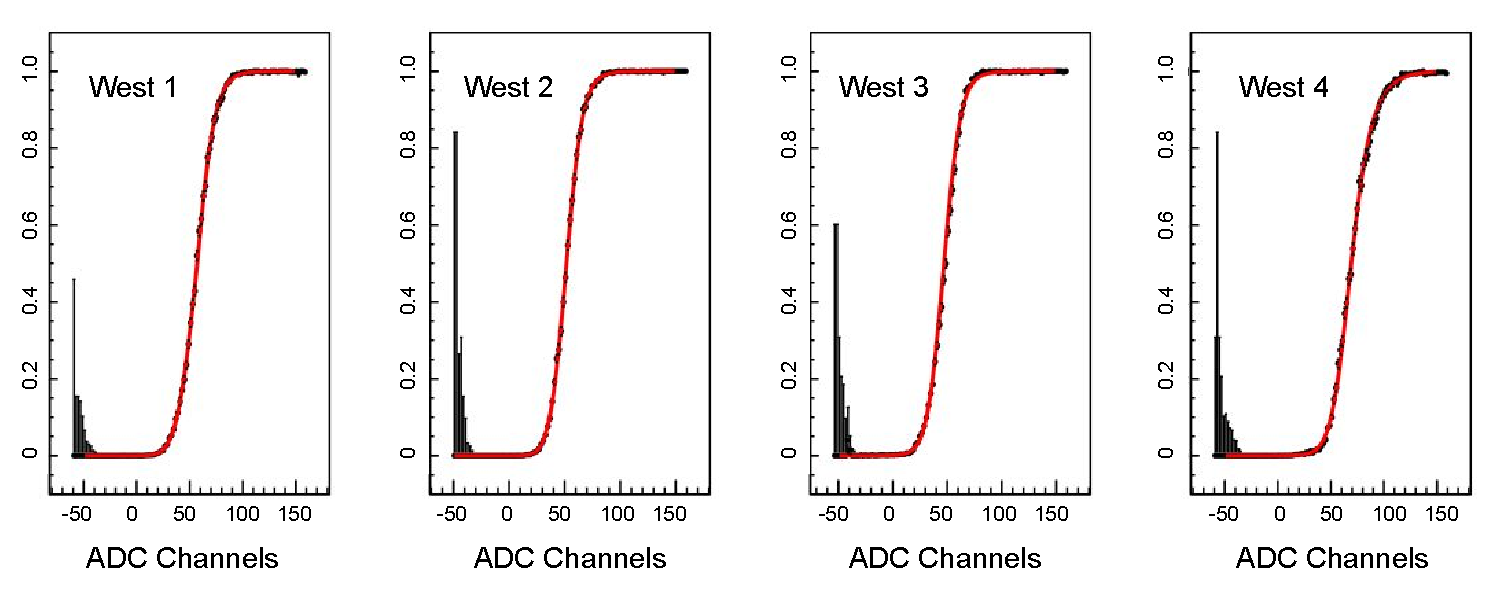
\includegraphics[scale=.6]{3-UCNAAnalysis/triggerThresholds.pdf}
\caption{Typical trigger thresholds as a function of pedestal subtracted
  ADC values from the West PMTs with fits shown in red. The y-axis
  is a probability of triggering given some ADC signal.}
\label{fig:trigger_thresh}
\end{figure}

\subsubsection{Functional Fit of the Trigger Threshold}
From the sigmoid shape of the threshold data in Figure \ref{fig:trigger_thresh}, one might guess
the shape of the curve to be a hyperbolic tangent or an error function. The data tends to show
a sharper turn on at lower ADC channels and a softer leveling off to unit probability, which
prompted the use of both the $\mathrm{erf}(x)$ (lower end of transition region)
and $\tanh(x)$ (upper end of transition region),
with a continuous transition between the
two provided by a smoothing function $S_\pm$ defined as
%
\begin{equation}
  S_\pm\big(x;x_0,R\big) \cdot f(x) = \frac{1}{2}\bigg(1\pm\tanh\Big(\frac{x-x_0}{R}\Big)\bigg) \cdot f(x),
\end{equation}
%
which acts to ``turn on/off'' ($+/-$) a function $f(x)$ around the pivot point $x_0$ and with the severity of
the on/off transition determined by the width parameter $R$. The functional fit $F(q)$ then becomes (note that the $\mathrm{erf}(x)$ and $\tanh(x)$ 
have the range (-1,1), so they must be shifted and the range halved to accommodate $0<F(q)<1$):
%
\begin{equation}
  F(q) = \frac{1}{2} \Bigg[ S_-\big(q;\mu,R\big) \bigg(1 + \mathrm{erf}\Big(\frac{q-\mu}{w_1}\Big)\bigg) +
  S_+\big(q;\mu,R\big) \bigg(1+\tanh\Big(\frac{q-\mu}{w_2}\Big)\bigg)\Bigg]
\end{equation}
%
where $q$ is the ADC value and
the free parameters are $\mu$ ($f(q=\mu)\approx 0.5$), $w_1$ (width of $\mathrm{erf}$), $w_2$ (width of $\tanh$), and $R$ (severity of turn on/off).
This function, while motivated purely by inspection of the shape of the trigger threshold, fits the data
quite well with only these four free parameters. An example of the fits for a single $\beta$-decay
run can be seen in Figure \ref{fig:trigger_thresh}. 

%-----------------------------------------------------------


\section{Simulation}
\label{sec:Simulation}

For this work, the simulation software from previous analyses was adopted
and modified where seen fit to accommodate changes in the geometries
and materials. The finer details of the particle generation and
tracking can be found in \cite{mpmThesis}. For our purposes, a summary
of the important quantities is sufficient for understanding
the work contained within this thesis.

\iffalse The simulations and application of the
detector response model provide a suitable starting
point for discussing the analysis, as the calibration of the data hinges
strongly on the simulation results. There is a notable dependence of the
response model on data, but this will be addressed as needed
when describing the calibration.

The simulation work for this thesis was completed
using the Geant4 simulation software package. The geometry of the
apparatus was duplicated
to the best precision possible and benchmarked against data after
the detector response model was applied. The structure
of the simulation code did not change from those in the previous analysis
as described in \cite{mpmThesis}, although minor changes were
made to the geometry to reflect real adjustments to the experimental
apparatus. \fi

\subsection{Overview}

The simulation of the experimental geometry and particle tracking was completed
using the \textsc{Geant4} Monte Carlo particle transport software package
\cite{agostinelli2003geant4}. The initial kinematics of the event vertices
were determined via a stand-alone kinematic event generator and fed into the \textsc{Geant4} toolkit, at which
point the particle was propagated via Monte Carlo sampling of interactions
with all components of the experimental geometry, including the magnetic field.
The energy deposition was recorded within all sensitive detector components and
even within the decay trap windows and walls, to which we do not have access
in the real data. The relative timing of the scintillator hits was also
recorded so as to mimic the timing signals of the experiment.

The simulation is especially important when determining systematic corrections due
to a priori knowledge of the initial kinematics of each event. Thus, after a particle
is stopped and its detector response is considered, one can compare the signature
of the signals to the initial momentum of the particle and analyze possible
effects on observables from backscattering, angular dependence, and energy losses
in non-sensitive detector regions for example.

\subsection{Geometry and magnetic field} \label{sssec:simMagField}

The geometry input into the \textsc{Geant4} simulation is taken directly from
that given in Chapter \ref{ch:UCNA_Experiment}. Options for each variation
of the geometry were implemented, including a 2011-2012 option with
the thicker decay trap endcaps and a 2012-2013 option with thinner asymmetric
decay trap endcaps. The 2012-2013 geometry is further subdivided into an option
for neopentane in the wirechamber (same as 2011-2012) and for isobutane in the
wirechamber, as a portion of the 2012-2013 runs were taken with this
different fill gas. Any other minor differences in the geometry were also
incorporated into the detector construction.

The magnetic field profile is nominally taken to be 1~T in the decay trap
with the field expansion to 0.6~T at the wirechambers incorporated also.
Options to use the measured field maps, one of which is depicted in
Figure \ref{fig:field_profile}, were included, but in all source
and $\beta$-decay simulations the smooth profile was used to save on
computation time. Effects on the asymmetry from the non-smooth
field profile present during data taking is addressed in
Section \ref{sssec:MagFieldSyst}.

The magnetic field is passed to the simulation as a set of discrete $B_z$
values along the $z$-axis of the spectrometer as depicted in Figure \ref{fig:field_profile}.
The continuous field profile on the $z$-axis is then interpolated between consecutive $z_i$ locations
using the respective $B_z(z_i)$ values by a half-wave of a cosine \cite{yuan2006progress},
%
\begin{equation}
  B_z(z) = \frac{B_z(z_i) + B_z(z_{i+1})}{2} + \frac{B_z(z_i) - B_z(z_{i+1})}{2}\cos\bigg(\frac{z-z_i}{z_{i+1}-z_i}\pi\bigg),
\end{equation}
%
where $z_i<z<z_{i+1}$.

Then, if the field is taken to be azimuthally symmetric ($B_\phi(z,r,\phi)=0$) and $B_z(z,r,\phi)=B_z(r)$,
the $r$-component can be calculated from Maxwell's equations:
%
\begin{equation}
  \nabla \cdot \vec{B} = 0 \Rightarrow \frac{\partial B_z}{\partial z} + \frac{1}{r}\frac{\partial}{\partial r}\big(rB_r\big), 
\end{equation}
\begin{equation}
  B_r(z,r) =  \frac{B(z_i) - B(z_{i+1})}{z_{i+1}-z_i}\frac{\pi r}{4}\sin\bigg(\frac{z-z_i}{z_{i+1}-z_i}\pi\bigg).
\end{equation}
%


\subsection{Event Kinematics}

\subsubsection{Conversion Electron Sources}
For the conversion electron sources, the decay probabilities for conversion electrons,
Auger electrons, and gamma rays are read from files specific to each isotope.
The energy and radiation type sample the decay chain probabilities from these files, and
the momentum is chosen isotropically over 4$\pi$. The initial vertex for any source
event is randomly sampled within a small dot ($\sim1.5$~mm) encapsulated in a model for a sealed source holder
along the center axis of the decay trap, as would be the case for a real sealed
source used in the calibration.

\subsubsection{Neutron $\beta$-decay Electrons} \label{sssec:betaSim}

A detailed account of the functional form of the unpolarized $\beta$-decay rate used in the
event generator
is given in \cite{mpmThesis}. The corrections to the plain phase space spectrum are taken from
Wilkinson's series of review articles on $\beta$-decay
\cite{wilkinson1982,wilkinson1989evaluation,wilkinson1990evaluation,wilkinson1993evaluation,
  wilkinson1995evaluation,wilkinson1997evaluation,wilkinson1998evaluation} and include
the Fermi function Coulomb correction, corrections for finite size of the nucleon, radiative
corrections as described in Section \ref{sssec:RadCorr}, and recoil corrections for the finite
mass of the proton in the final state.

For this analysis, the decays were sampled from a polarized spectrum, thus necessitating the
addition of the asymmetry to the decay rate. The polarized decay rate then took the form:
\begin{equation}
  \Gamma^{\mathrm{pol}}_\pm(E) = \Gamma^{\mathrm{unpol}}(E_e) \bigg( 1 \pm \xi(E) \bigg),
\end{equation}
where
\begin{equation}
  \xi(E) = A(E)\Big(1+\mathrm{R.O.}(E)+\mathrm{Rad}(E)\Big),
\end{equation}
$A(E)=A_0\beta \cos\theta$, ``R.O.'' and ``Rad'' are the recoil order and radiative corrections to the asymmetry
consistent with those from Sections \ref{sssec:ROCorr} and \ref{sssec:RadCorr}, $\pm$ indicates the two possible spin states,
and $\Gamma^{\mathrm{unpol}}$ is the unpolarized
spectrum. The value of $A_0= -0.1184$ was used, as this was the global average at the time of the simulation
development \cite{pdg}.


Each spin state was simulated for the 2011-2012 geometry, 2012-2013 geometry with neopentane in the wirechamber,
and 2012-2013 geometry with isobutane in the wirechamber. Matching the proper spin state simulation to the polarization orientation
in the $\beta$-decay runs allows one to analyze the simulated data identically to the data. By comparing the
extracted asymmetries to the input value of $A_0$, we can ensure that the analysis method is at least internally
consistent.

It should be noted that including the asymmetry in the initial probability distribution
is a new contribution to the analysis, as in past analyses the electrons were generated from the unpolarized
spectrum and then the final spectra were weighted by the above asymmetry factor $\xi(E)$.
A special thanks is in order for X. Sun for his contributions to the polarized event generator.

\subsection{Output}
The \textsc{Geant4} simulation provides trajectory tracking along with
the energy deposition along these tracks. Prior to processing the simulation
for calibration or systematic purposes, the first
task is to construct observables that are more useful.

\subsubsection{Energy Deposition}
By tallying the energy deposited along an entire track within some subset
of the geometry, one can reconstruct the energy deposited anywhere within
the SCS. The areas of primary interest for the sake of analysis are the
wirechambers and the scintillators. The energy deposited in the scintillator
is of highest importance, as the systematic studies depend on scintillator
reconstructed energy.  From here on,
the energy lost in the scintillator, as determined from summing the energy loss in simulation, will be
referred to as $E_{\mathrm{dep}}$. This is the maximum energy which could be detectable
for an event if no inconspicuous energy losses existed.

\subsubsection{Quenched Energy} \label{sssec:Equenched}
In reality, the energy that is visible in the form of scintillation light is not exactly
equal to $E_{\mathrm{dep}}$, but rather some of the energy is ``quenched'' when
the energy deposition per unit length grows large near the end of a track. The
empirical description for the light output by a charged particle traversing a
scintillator is given by Birk's Law \cite{birks1951scintillations}:
%
\begin{equation}
  \frac{dL}{dx} = S\frac{\frac{dE}{dx}}{1+k_B\frac{dE}{dx}},
\end{equation}
%
where $dL/dx$ is the light output per unit length, $dE/dx$ is the energy deposited per unit
length, $S$ is the scintillation efficiency, and $k_B$ is Birk's constant which must be
determined through measurement. For small $dE/dx$,
$dL/dx \propto dE/dx$, which is the case for the majority of an electron's track inside the scintillator.
As the electrons slow down and become very low energy, $dE/dx$ increases drastically
and $dL/dx \approx S/k_B = constant$. It is precisely this quenching effect that creates the difference
between the deposited energy and energy that may be observed through scintillation light. The energy
proportional to $dL/dx$ will be called the quenched energy and is defined as
%
\begin{equation}
  E_Q = \int \frac{\frac{dE}{dx}}{1+k_B\frac{dE}{dx}}dx,
\end{equation}
%
with the integration performed over the entirety of the path.

\begin{figure}[h] 
\centering
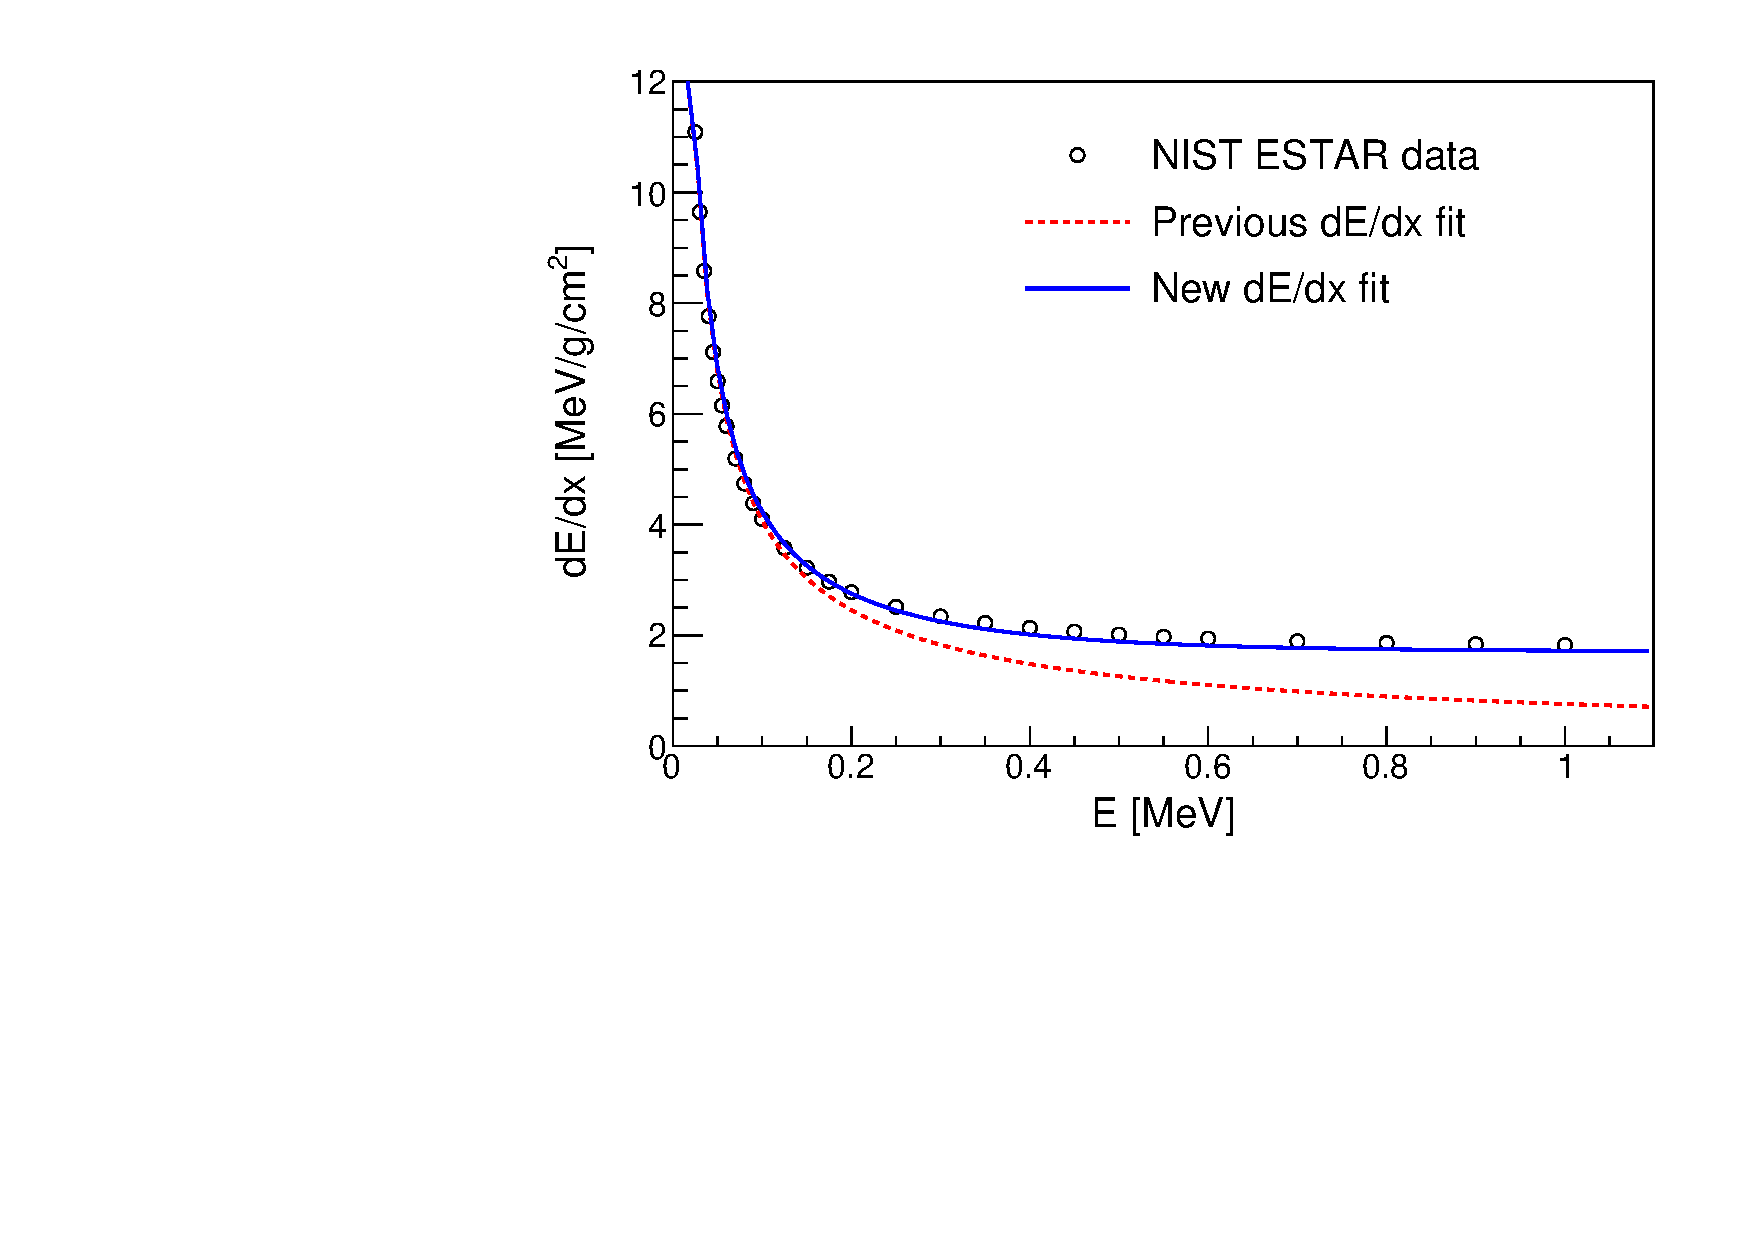
\includegraphics[scale=.6]{3-UCNAAnalysis/dEdx.pdf}
\caption{Plot of $dE/dx$ for a plastic scintillator. The data (open circles) comes from NIST ESTAR,
  and the $dE/dx$ functional forms used previously (red dashed line) and presently (blue solid line)
  are shown.}
\label{fig:dEdx}
\end{figure}

In previous analyses, the functional form of $dE/dx $ was extracted from a fit to NIST ESTAR data
for a plastic scintillator \cite{yuan2006progress}. The fit determined the following relationship:
%
\begin{equation}
  \frac{dE}{dx} = 116.7\bigg(\frac{E}{\mathrm{keV}}\bigg)^{-0.7287} \rho_{\mathrm{scint}} \frac{\mathrm{MeV}}{\mathrm{g/cm}^2},
\end{equation}
%
where $\rho_{\mathrm{scint}}=1.032~\mathrm{g/cm}^2$ is the density of the scintillator. From
inspection of Figure \ref{fig:dEdx}, one can see that this expression for $dE/dx$ (red dashed line)
does not fit the data well at higher particle energy. Thus Dr. Brad Filippone suggested that the
functional form previously used be modified \cite{bradF_ELOG}:
%
\begin{equation}
  \bigg(\frac{dE}{dx}\bigg)_{\mathrm{new}} = \bigg(\frac{dE}{dx}\bigg)_{\mathrm{old}} + 1.35\big(1-e^{-0.00125\frac{E}{\mathrm{keV}}}\big) \rho_{\mathrm{scint}} \frac{\mathrm{MeV}}{\mathrm{g/cm}^2},
\end{equation}
%
which produces much better agreement with the data in Figure \ref{fig:dEdx}. The new $dE/dx$ was implemented for calculations
of $E_Q$ in the \textsc{Geant4} simulation for the current analysis with the value of $k_B=0.0191\pm0.0020$~cm/MeV as determined in
\cite{yuan2006progress}.




\subsubsection{Position of Detector Hits}
The detector positions in both the scintillator and wirechamber are calculated as the weighted
average of the step positions, with the weights equal to the energy deposited in that step.
A more detector-like position response was utilized when analyzing the simulated data as is described
in Section \ref{ssec:simWirePos}, where the same position reconstruction algorithm used for data
is applied to simulated wirechamber responses.


%----------------------------------------------------------

\section{Energy Response from Detector Response} \label{sec:EnergyResponse}

The visible energy $E_{\mathrm{vis},i}$ deposited
in the scintillator as seen by a single PMT $i$ for an event at position $(x,y)$ 
is given by the following: 

\begin{equation} \label{eq:EvisResponse}
E_{\mathrm{vis},i} = \eta_i^{-1}(x,y) \cdot f_i\bigg( \Big( \mathrm{ADC}_i - p_i(t) \Big) \cdot g_i(t) \bigg)  ,
\end{equation}

\noindent where 
\begin{align*}
  f_i(\mathrm{ADC}) = & \text{ linearity relation from pedestal subtracted and gain corrected} \\
  & \text{ ADC values to a quantity proportional to scintillation} \\
  & \text{ light reaching PMT \textit{i} (see Section \ref{ssec:linCurves}),}\\
  \eta_i(x,y) = &\text{ PMT position dependent response factor to correct for} \\
    & \text{ position dependence of light response (see Section \ref{sssec:posmaps}),} \\
  p_i(t) = &\text{ mean pedestal value for PMT } i \text{ (see Section \ref{ssec:pedSubtraction}),} \\
  g_i(t) = &\text{ gain correction factor for PMT }i \text{ (see Section \ref{ssec:BiGain})}.
\end{align*}

This expression is exact in the case where all values are determined with infinite
precision and without stochastic fluctuations. Unfortunately, each parameter on the right
side of this equation is either stochastic in itself (as is the ADC response), or it was
determined via observation of a random process (the gain and pedestal), and so
the underlying value for any given event may not be the same as the value applied in the
above expression. Thus what we
really resolve is an approximation to the energy, which comes with some uncertainty. The uncertainty
on the asymmetry that results from imperfect energy determination
will be addressed in Section \ref{ssec:energyRecon}.


\subsection{Combining PMT Responses} \label{ssec:combinePMT}

For every two-fold trigger, all four PMTs from each side (eight in total) are read out by the
DAQ. Upon application of the individual detector calibrations, this yields
eight visible energies, $E_{\mathrm{vis},i}^\mathrm{E,W}$, where $i$ runs from 1 to 4 for the
four PMTs on each side. For each detector, the four available energies should
be combined to create a visible energy for each side, $E_{\mathrm{vis}}^\mathrm{E,W}$. While the
majority of events only strike one scintillator so only one of the E/W visible energies will
be useful, the Type 1 events will have a usable energy on each side.

Now not all PMTs behave identically Some PMTs have better resolution than others, thus these PMTs
should contribute more to the average energy. A simple average would not account for this, but
a weighted average, upon definition of the weights, will suffice:
%
\begin{equation}
  E_{\mathrm{vis}}^\mathrm{E,W} = \frac{\sum_{i=1}^{4} w_i E_{\mathrm{vis},i}^{\mathrm{E,W}}}{\sum_{i=1}^{4} w_i},
\end{equation}
%
where $w_i=\frac{1}{\sigma_i^2}$ are the weights for each $E_{\mathrm{vis},i}^{\mathrm{E,W}}$. We will drop the superscript
E/W for now, understanding that what follows is done for each detector.

Now let's assume that the $E_{\mathrm{vis},i}$ from Equation \ref{eq:EvisResponse} is an approximation
for an event which deposited exactly the energy $E_Q$ (the $Q$ stands for ``quenched'', which will
be described in Section \ref{sssec:Equenched}). A certain amount of this $E_Q$ is visible to each
PMT, given by $\eta_i(x,y)E_Q$, as each PMT only captures a portion of the total number of photons produced
in the scintillator.
Now if we want to relate this to the signal read out by the DAQ
from the PMT, we must multiply by a PMT resolution factor $\alpha_i$ to convert from energy
to photoelectrons, giving $N_i = \alpha_i \eta_i(x,y) E_Q$.
These PMT resolution factors are calculated during the calibration process
and will be discussed in Section \ref{ssec:PMTresolution}, but for now, assume they are known.

The number of photoelectrons produced by a PMT is a stochastic process, so we can write the actual
measured number of photoelectrons as $\overline{N_i} = N_i \pm \sqrt{N_i}$. The fractional uncertainty
is then $1/\sqrt{N_i} = 1/\sqrt{\alpha_i \eta_i(x,y) E_Q}$. Now, since the measured number of photoelectrons,
$\overline{N_i}$, is directly proportional to the ADC signal of the PMT and thus also the visible energy
of the PMT by Equation \ref{eq:EvisResponse}, we have
%
\begin{equation}
  E_{\mathrm{vis},i} = E_Q \pm \frac{E_Q}{\sqrt{\alpha_i \eta_i(x,y) E_Q}} =  E_Q \pm \sqrt{\frac{E_Q}{\alpha_i \eta_i(x,y)}}.
  \label{eq:Evisi}
\end{equation}
%

The measured value of $E_{\mathrm{vis},i}$ is actually sampled from a distribution with $\mu$ and $\sigma$ given by the
above equation, but we can assume that the best weight is given by $w_i = \frac{1}{\sigma_i^2} = \frac{\alpha_i \eta_i(x,y)}{E_Q}$.
Then the final combined $E_{\mathrm{vis}}$ for a single detector becomes
%
\begin{align}
  E_{\mathrm{vis}} &= \frac{\sum_{i=1}^{4} \frac{\alpha_i \eta_i(x,y)}{E_Q} E_{\mathrm{vis},i}}{\sum_{i=1}^{4} \frac{\alpha_i \eta_i(x,y)}{E_Q}}
  = \frac{\sum_{i=1}^{4} \alpha_i \eta_i(x,y) E_{\mathrm{vis},i}}{\sum_{i=1}^{4} \alpha_i \eta_i(x,y)} 
  = \frac{\sum_{i=1}^{4} \alpha_i f_i(q)}{\sum_{i=1}^{4} \alpha_i \eta_i(x,y)}
\end{align}
%
where we have used Equation \ref{eq:EvisResponse} with $q=\big( \mathrm{ADC}_i - p_i(t) \big) \cdot g_i(t)$.
The uncertainty on the final weighted average above is given by
\begin{equation}
  \delta E_{\mathrm{vis}} = \frac{1}{\sqrt{\sum_{i=1}^{4} w_i}} = \frac{1}{\sqrt{\sum_{i=1}^{4} \frac{\alpha_i \eta_i(x,y)}{E_Q}}}
    \approx  \sqrt{\frac{E_{\mathrm{vis}}}{\sum_{i=1}^{4}\alpha_i \eta_i(x,y)}}.
\end{equation}
This is only approximately the uncertainty since $E_Q$ must be replaced by the energy estimate $E_{\mathrm{vis}}$. The quenched
energy is not a known quantity within data and is precisely the quantity being estimated, thus it cannot
be present in the uncertainty if it is to be calculated for data. This approximation has no impact
on the analysis though, as the calculation of the impact of the energy uncertainty on the final asymmetry is unrelated
to $ \delta E_{\mathrm{vis}}$ (See Section \ref{ssec:energyRecon}).

As pointed out in \cite{mpmThesis}, the position map values only enter into the weighted average
as part of the sum in the denominator and multiplied by the $\alpha_i$ conversion factors, which is a smoother
function of position than the individual position map values, and thus sensitivity to uncertainty in position map
values $\eta_i$ should be minimized.

\subsection{$E_{\mathrm{vis}}$ to $E_{\mathrm{recon}}$}

As mentioned in Section \ref{sec:outline}, $E_{\mathrm{vis}}$ is an estimate of the
energy visible to the PMT from deposition in the scintillator. The more useful
initial energy of the particle must be determined using a separate parameterization.
To determine such a parameterization, simulated data is used so that the initial
energies of the events are known exactly, and then the response of the detector
to different event energies and types can be investigated.

\begin{figure}[h]
  \centering
  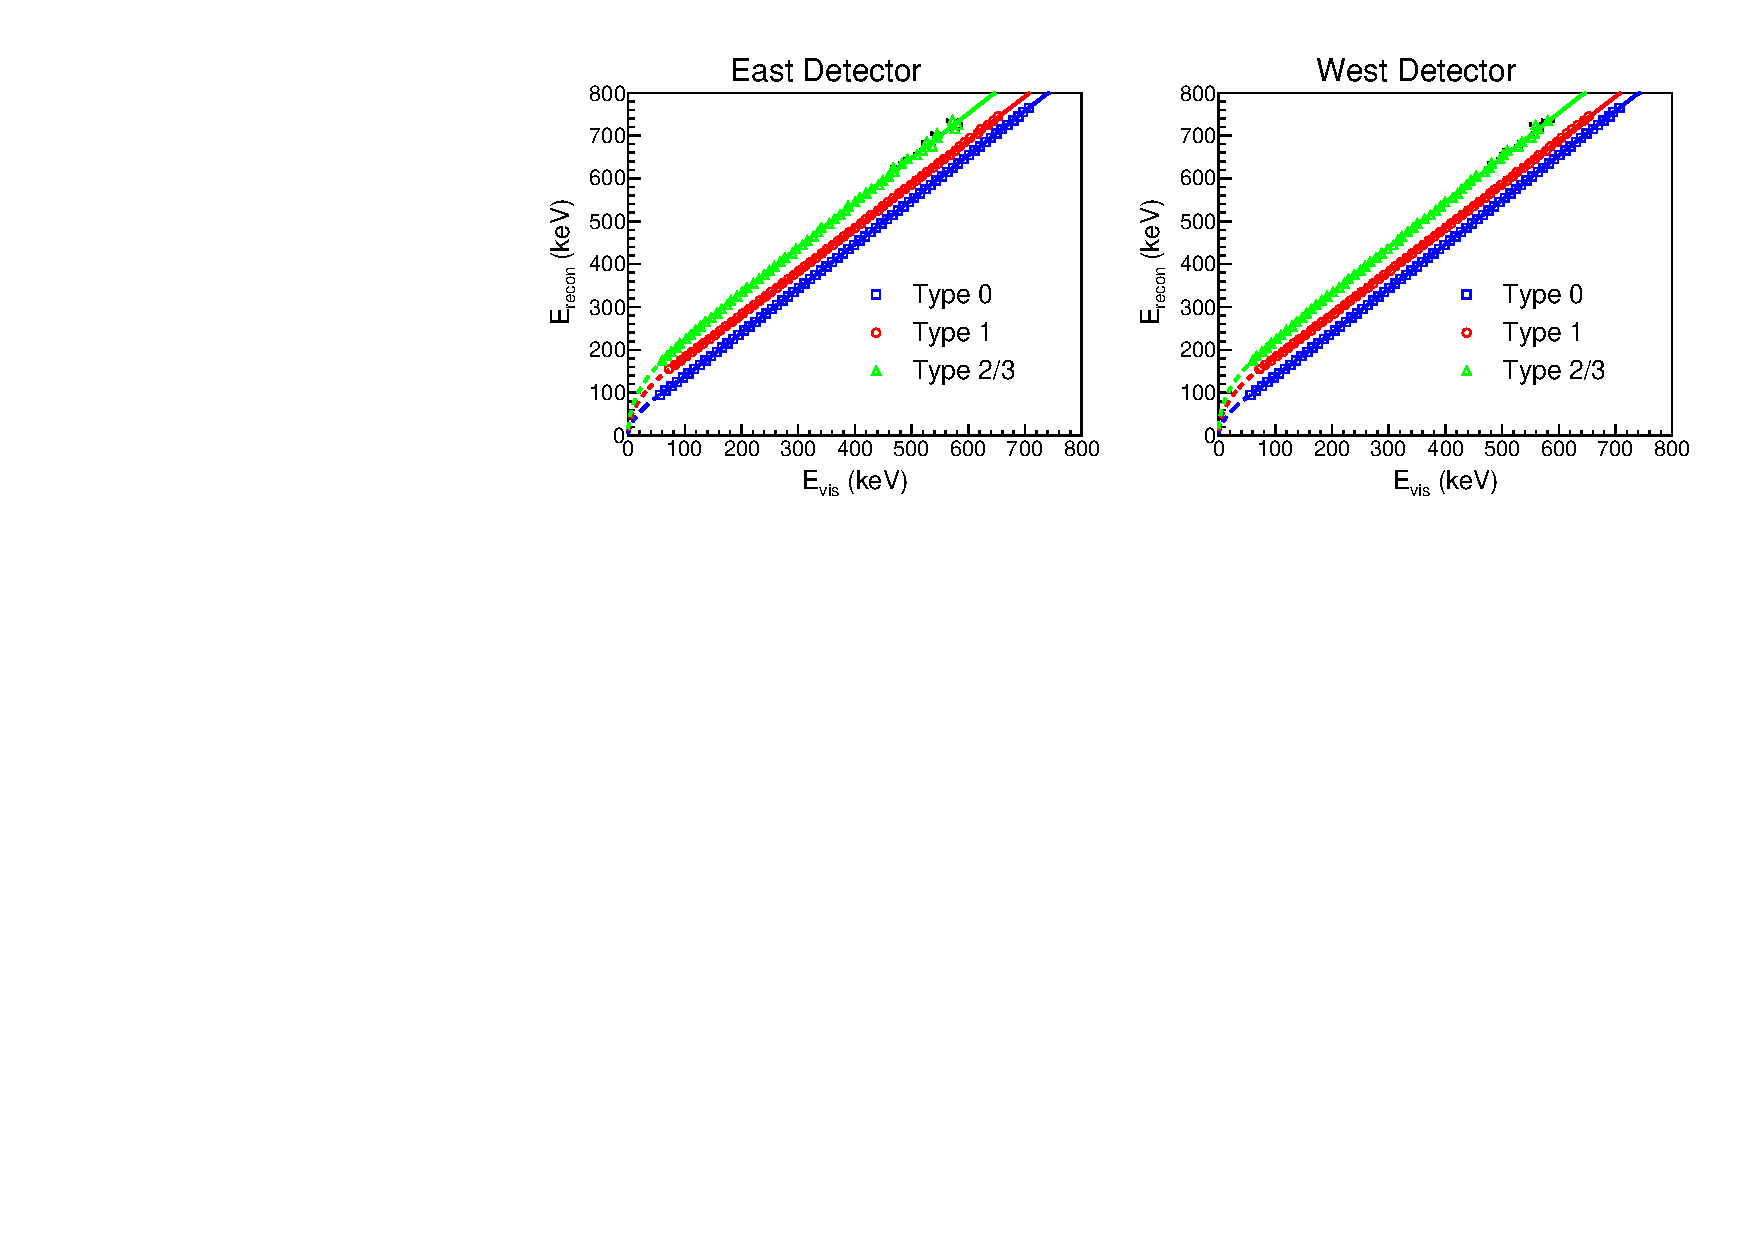
\includegraphics[scale=0.78]{3-UCNAAnalysis/2011-2012_Evis_to_Erecon.pdf}
  \caption{Parameterization between $E_{\mathrm{vis}}$ and $E_{\mathrm{recon}}$ for the 
    2011-2012 geometry, as determined from simulation.
    The mapping for the other geometries are very similar and thus are
    not shown.}
  \label{fig:Erecon}
\end{figure}

The mapping between $E_{\mathrm{vis}}$ and $E_{\mathrm{recon}}$ is determined separately
for 2011-2012, 2012-2013, and 2012-2013 with isobutane in the wirechamber.
Using the simulated $\beta$-decay spectrum and a characteristic set of detector
response variables, the simulated events are processed in the same manner as
they would be for data. They are identified as Type 0, 1, or 2/3, and their
$E_{\mathrm{vis}}$ values for each detector are determined. Then the events are
grouped into histograms using their initial energy (we will call it $E_{\mathrm{recon}}$,
but really this is the true energy of the events), with the histogram bins corresponding
to 10~keV groups from 0~keV to 790~keV. Then each of these histograms are fit to
determine the average $E_{\mathrm{vis}}$ value for a given $E_{\mathrm{recon}}$. The results
of these fits for each event type in each detector for 2011-2012 is shown as the data
points in Figure \ref{fig:Erecon}. The other geometries look very similar and thus are
left out. Data points with low statistics at low energies were dropped.

The fit to the data is of the form
\begin{equation}
  E_{\mathrm{recon}} = C_1 + C_2E_{\mathrm{vis}} + \frac{C_3}{E_{\mathrm{vis}}} + \frac{C_4}{{E_{\mathrm{vis}}}^2},
\end{equation}
and then the fit is extrapolated continuously to zero from the lowest energy data point using
\begin{equation}
  E_{\mathrm{recon}} = C_5{E_{\mathrm{vis}}}^{C_6}
\end{equation}
with the parameters $C_5$ and $C_6$ determined by ensuring the two equations are equal at the
transition point along with their first derivatives. The reason for the linear relationship
can be attributed to the low energy quenching effects as described in Section \ref{sssec:Equenched}.
As $E_{\mathrm{recon}}$ becomes small, a larger proportion of the electron's energy is affected by quenching, and thus
the lower energy events exhibit this nonlinear behavior.

Using the fitted parameters, an $E_{\mathrm{recon}}$ value is determined
for every event by plugging its weighted average $E_{\mathrm{vis}}$ into the proper equation.
It should be noted that for Type 1 events, the visible energies of both the East and West
detectors are added together when determining the parameterization, so
the same is done when applying the above parameterization to data. This is done to utilize as much
detector information as possible. The side for a Type 1 event is set to
the detector with the earlier trigger, making it the primary detector.
Thus, for a Type 1
event, one would plug $E_{\mathrm{vis}} = E_{\mathrm{vis}}^E + E_{\mathrm{vis}}^W$ into the $E_{\mathrm{recon}}$
equation for the side that triggered first.

\section{Detector Response Model} \label{sec:DetectorResponseModel}
The goal of the Detector Response Model is to create an estimate of the potential PMT
signals from the $E_Q$ produced in the simulation. While it is true that the simulation
captures the true physics of the experiment, the simulation output does not properly
represent the data signals.
For instance, the purely simulated scintillator energy depositions have sharp peaks at the
maximum allowed energy deposition with low
energy tails, a result of energy losses elsewhere in the apparatus. The less probable outer shell
conversion electron lines are also visible in the simulation. The data signals
on the other hand are smeared out in a Gaussian fashion, with no possible
resolution of the outer shell electron lines due to the resolution of the detectors not
being sufficiently narrow.
The Gaussian-like peaks arise from finite resolution effects and
must be incorporated in the simulatin using parameters calculated
from real data.  


\subsection{Extracting simulated ADC values}


Recall from Section \ref{sec:EnergyResponse} that we can relate a PMT signal,
$\mathrm{ADC}_i$, to the energy deposited in the scintillator
using Equation \ref{eq:EvisResponse}.
Our goal is to reverse engineer this expression to write an ADC signal as a
function of the visible energy, noting that the visible energy is directly
related to the quenched energy from simulation. Directly from \ref{eq:EvisResponse}
we can trivially write down:
%
\begin{equation} \label{eq:pmtResponse}
\mathrm{ADC}_i = f_i^{-1}\big(\eta_i(x,y) E_{\mathrm{vis},i} \big)/g_i + p_i
\end{equation}
%
where we have dropped the time dependence for brevity. For the time being, take
the PMT response functions $f$ and the position dependent response values $\eta_i(x,y)$ to be known,
as their determination is addressed in Sections \ref{ssec:linCurves} and \ref{sssec:posmaps}
respectively.

Now we can further generalize this expression by recalling that the gain and the pedestals
were extracted from distributions, with the values used in the gain correction and pedestal
subtraction equal to the mean of the distribution. Technically speaking though, there is a
well-defined probability that the actual gain and pedestal were not equal to this mean, but rather
sampled some other value from the distributions. To account for this, we will add a spread
to the gain and pedestal:
%
\begin{equation} 
  \mathrm{ADC}_i = f_i^{-1}\big(\eta_i(x,y)  E_{\mathrm{vis},i} \big)/\big(g_i\pm\delta g_i\big) + \big(p_i \pm \delta p_i\big).
  \label{eq:pmtResponse}
\end{equation}
%
This is to be interpreted as the pedestal (gain) being sampled from a normal
distribution with mean $p_i$ ($g_i$) and sigma $\delta p_i$ ($\delta g_i$).

Remember the goal is to plug in $E_Q$ and return an ADC value for each PMT, so we must next
relate $E_Q$ to $E_{\mathrm{vis}}$. What we really need is an expression for $\eta_iE_{\mathrm{vis}}$ in terms of $E_Q$.
Backtracking for a moment, we recall that $E_{\mathrm{vis}}$ is by definition the result
of plugging the ADC response into equation \ref{eq:EvisResponse}. The ADC response is proportional to the final amount of charge
that reaches the anode in a PMT, and is thus the product
of several stochastic processes and is only an estimate of the initial light from the scintillator that reached
the photocathode. In fact, every dynode within the photomultiplier introduces stochasticity into the process, as every time an electron
strikes a dynode, the number of emitted electrons is Poisson distributed. The final number of electrons that reach the anode
can be expressed as several nested Poisson distributions,
with the initial number of electrons (the input of the first nested Poisson process)
equal to the number of photoelectrons present at the photocathode. The series of Poisson
processes randomizes the final number of electrons seen by the anode, and therefore randomizes the ADC response.

Let us attempt to estimate the total number of electrons that reach the anode, which in turn yields something
proportional to the ADC response and thus also related to $E_{\mathrm{vis}}$. We will use only two nested Poisson
processes, where the first emulates the gain from the very first dynode, and the second captures the gain from the rest of
the dynodes as a whole. We then have:
%
\begin{equation}
  N_i^{\mathrm{tot}} \approx \mathrm{Pois}(g_r \cdot \mathrm{Pois}(g_d \cdot N_i)),
  \label{eq:ntot1}
\end{equation}
%
where $N_i^{\mathrm{tot}}$ is the total number of electrons to reach the PMT anode, $g_d$ is the gain of the first dynode,
$g_r$ is the total gain of the rest of the dynodes, and $N_i$ is the number of initial photoelectrons at the photocathode.
This number of photoelectrons is precisely related to the amount of light which reaches the PMT, which as a matter of fact
we defined as $N_i = \alpha_i \eta_i(x,y) E_Q$ in Section \ref{ssec:combinePMT}. Here $\alpha_i$ is again the PMT resolution
factor which relates the number of photoelectrons to energy, and for now we should take it as known (see Section
\ref{ssec:PMTresolution}).

Rewriting Equation \ref{eq:ntot1} we have
\begin{equation}
  N_i^{\mathrm{tot}} \approx \mathrm{Pois}(g_r \cdot \mathrm{Pois}(g_d \cdot \alpha_i \eta_i(x,y) E_Q)).
  \label{eq:ntot2}
\end{equation}
Here $N_i^{\mathrm{tot}}$ is an estimate of the total number of electrons that reach the PMT anode, but we can turn it
into an estimate of the number of initial photoelectrons simply by dividing by each of the dynode gain factors:
\begin{equation}
  \overline{N_i} \approx \frac{1}{g_rg_d}\mathrm{Pois}(g_r \cdot \mathrm{Pois}(g_d \cdot \alpha_i \eta_i(x,y) E_Q)).
  \label{eq:ntot3}
\end{equation}

But now we should realize that we already have an expression for $\overline{N_i}$ from Section \ref{ssec:combinePMT}, namely
\begin{align}
  \overline{N_i} &= N_i \pm \sqrt{N_i} \\
  &= \alpha_i \eta_i(x,y) E_Q \pm \sqrt{\alpha_i \eta_i(x,y) E_Q} \\
  &= \alpha_i \eta_i(x,y) \Bigg( E_Q \pm \sqrt{\frac{E_Q}{\alpha_i \eta_i(x,y)}}\Bigg) \\
  &= \alpha_i \eta_i(x,y) E_{\mathrm{vis},i} 
  \label{eq:bam}
\end{align}
where we used Equation \ref{eq:Evisi} in the last line. Thus we can now write
\begin{equation}
   \alpha_i \eta_i(x,y) E_{\mathrm{vis},i} \approx \frac{1}{g_rg_d}\mathrm{Pois}(g_r \cdot \mathrm{Pois}(g_d \cdot \alpha_i \eta_i(x,y) E_Q)),
  \label{eq:ntot4}
\end{equation}
directly from which our desired expression for $\eta_i(x,y) E_{\mathrm{vis},i}$ follows:
\begin{equation}
   \eta_i(x,y) E_{\mathrm{vis},i} \approx \frac{1}{\alpha_i g_rg_d}\mathrm{Pois}(g_r \cdot \mathrm{Pois}(g_d \cdot \alpha_i \eta_i(x,y) E_Q)).
  \label{eq:etaEvis}
\end{equation}

The last outstanding question is then what values to use for the gain of the dynodes. The PMTs are
Hamamatsu model R7725, run typically between 1100-1300~V. From the Hamamatsu documentation \cite{hamamatsu},
this model PMT has a total gain of $\sim2\times 10^5$ when run at $\sim1100$~V. Since this PMT has 12 stages (dynodes),
if we assumed equal gain on every dynode this would give $g_d\approx2.7$. But the first dynode is biased $4\times$ higher
than the rest, so it should exhibit a higher gain. Thus the gain of the first dynode was set to $g_d=16$, which then determines
that the gain of the rest of the dynodes combined should be $g_r = 2\times 10^5/g_d = 12500$.

\subsection{Applying the Detector Response Model}

With Equation \ref{eq:etaEvis} to approximate $\eta_i(x,y) E_{\mathrm{vis},i}$ for each PMT, this can be plugged into
$f^{-1}$ to return an initial ADC estimate in the form of Equation \ref{eq:pmtResponse}. The gain and pedestal
widths could be taken as zero without substantial loss of model integrity, as the majority of the detector
response has been captured using the position dependent response, PMT resolution factors, and sampling of the
Poisson processes. The gain is stable enough that including a sampling of the width introduces $<1\%$ fluctuations
in modeled ADC, and so it was ignored. The pedestal distributions for each PMT were sampled and used in the
Detector Response Model, as this gives a width to a signal with no energy deposition as is seen in the data.
To apply the random sampling of the pedestal, a Gaussian is randomly sampled with mean equal to zero and sigma equal
to the rms recorded for that PMT in the run of interest. This random value is then added to the ADC estimate. 

Once all $\mathrm{ADC}_i$ have been calculated, the two-fold trigger model must be applied.
The PMT trigger thresholds as determined in Section \ref{sec:triggerThresh} are retrieved for the run of interest.
The probability of triggering is read from the trigger threshold function for an individual PMT, and then
acceptance/rejection is performed to decide whether the PMT triggered. The basic two-fold trigger logic is
applied, so if two or more PMTs trigger, the scintillator on that side is recorded as having a two-fold trigger.

With the modeled $\mathrm{ADC}_i$ values calculated and the pedestal width sampled and added to the signal, the ADC values
are treated as though they are data and plugged into Equation \ref{eq:EvisResponse}. This subtracts the mean pedestal,
applies the gain correction, and then maps the ADC response back to a new estimate of $\eta_i(x,y) E_{\mathrm{vis},i}$
using the calibration linearity curve $f_i(\mathrm{ADC})$. Upon dividing by the position dependent light transport
value $\eta_i(x,y)$, one has estimates for the visible energies from all PMTs.

At this point, the individual $E_{\mathrm{vis},i}$ are combined using the now familiar methods of Section \ref{ssec:combinePMT}.
Then a final $E_{\mathrm{recon}}$ value is determined via the normal parameterization. Everything about the simulation event
now resembles a data event, and thus the analysis procedure for data and simulation becomes identical.




%---------------------------------------------------------------------------------------


\section{Calibration Overview}

In the next chapter, we will take an in depth look at the calibrations of both
the wirechamber and the scintillator. Here we simply highlight their use in the analysis.

\subsection{PMT Calibration} \label{ssec:PMTCal}

The PMT calibration, as mentioned in Section \ref{sssec:scintEnCal},
uses well known conversion electron sources
to understand the detector response to their well-defined energies. By comparing the detector
response (coupling both ADC values and position map values) to simulated responses,
we can map ADC signals from each PMT to visible energies deposited
in the scintillator. These calibrations parameterize the detector response so that the
functional form of the calibration can be applied to the $\beta$-decay data.

\subsection{Wirechamber Calibration}

The wirechamber calibration relates the anode signal in the MWPC to an energy deposited in the MWPC. This is
primarily useful for separating the Type 2/3 backscattering events, as the
energy deposition in the MWPC is not used within the reconstruction of an electron's initial
energy. This separation is important though as it drastically reduces the systematic
correction for these backscattering events.
 

\section{Polarimetry} \label{sec:polarimetry}

The polarimetry analysis was carried out by Eric Dees of North Carolina State University and
deserves the attention of an entire dissertation itself. The previous polarimetry measurement
is described in detail in a dissertation by Adam Holley \cite{holley2012ultracold}. A major
difference between the previous depolarization measurement and the current depolarization
hinges upon the installation of the shutter between the spin flipper and decay trap. An
update of the new polarimetry measurement method can be found in the publication of the result
presented within this dissertation \cite{brown2017}.

\begin{figure}[h] 
\centering
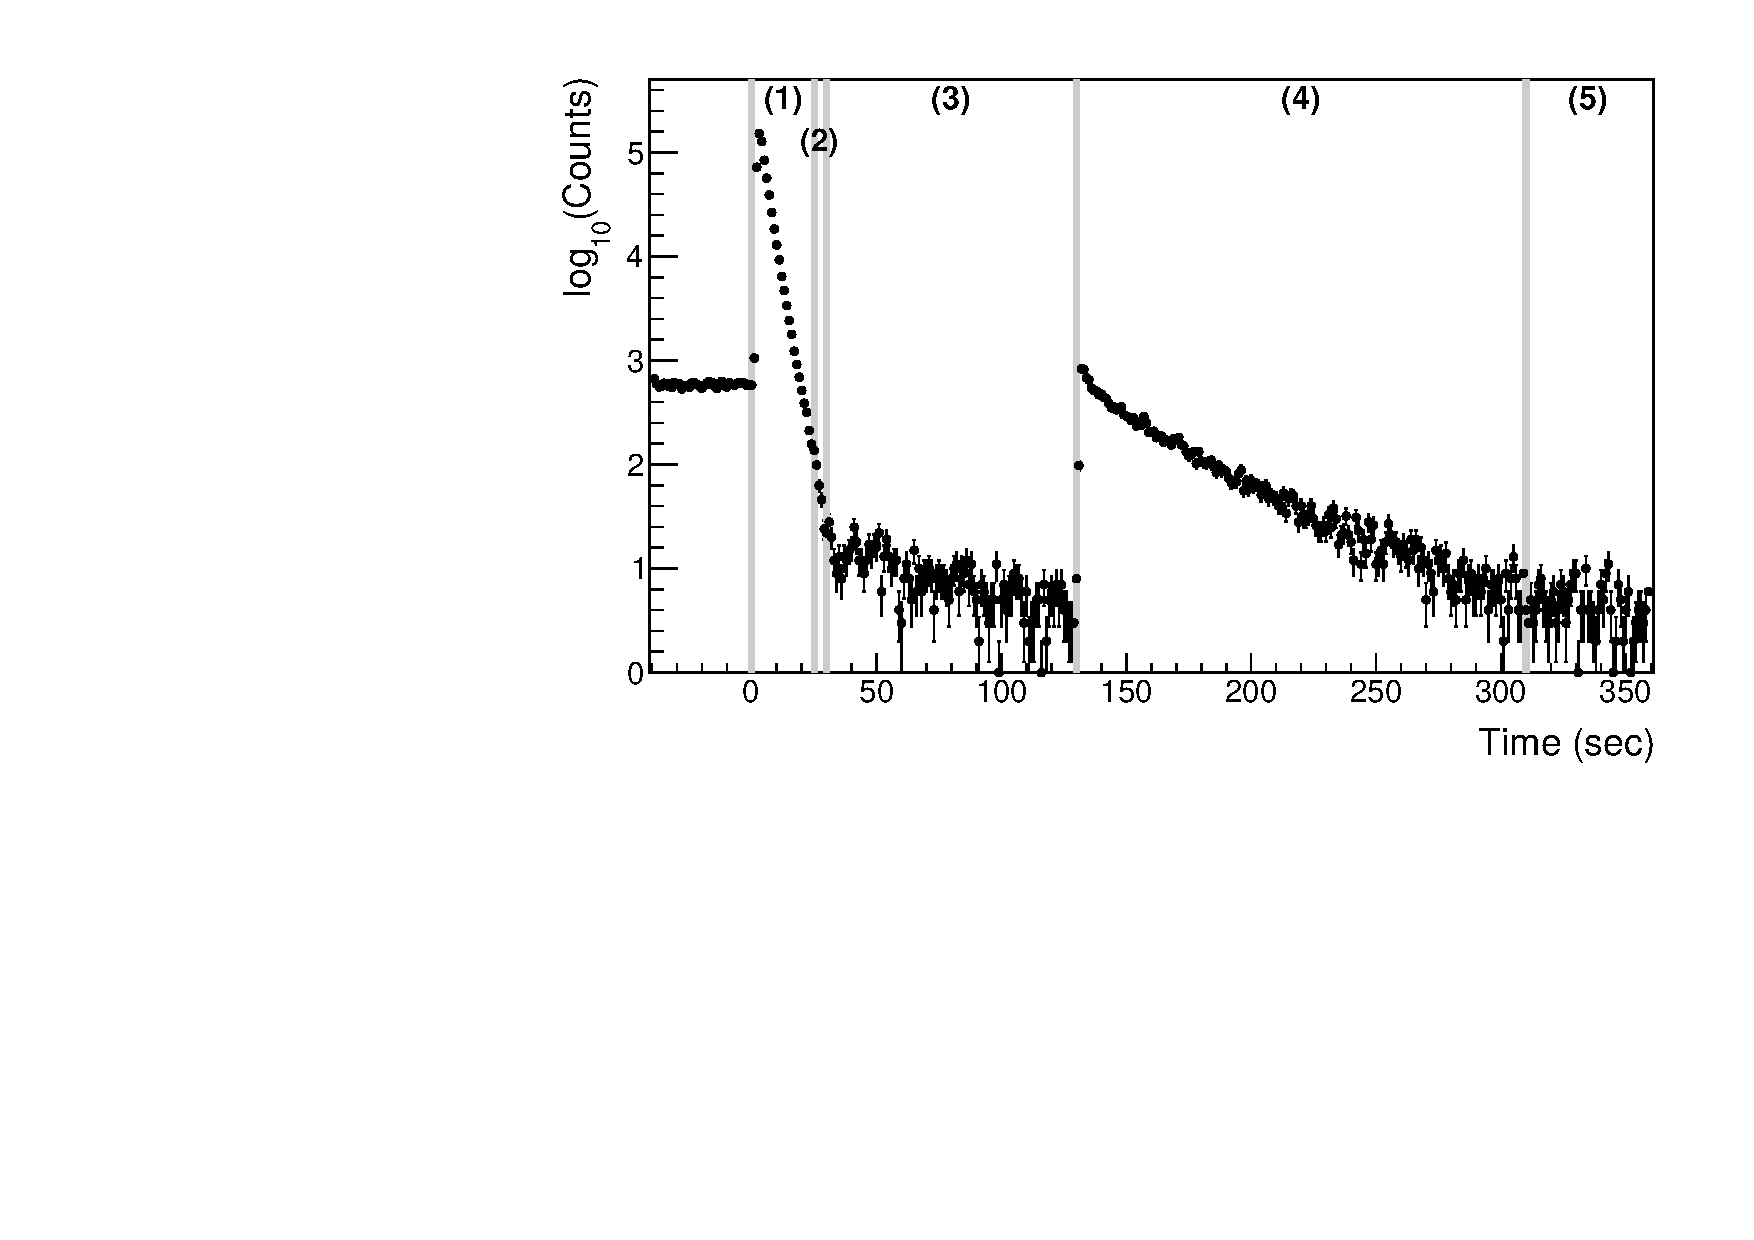
\includegraphics[scale=.55]{3-UCNAAnalysis/Switcher_signals.pdf}
\caption{Figure courtesy of E. Dees and A. R. Young as published in \cite{brown2017}.
  ``Switcher signal as a function of time, during ``D''-type runs: (1) the shutter
  closes and the switcher state changes, permitting UCN in the
  guide outside the decay volume to drain to the switcher UCN detector, (2) the AFP
  spin-flipper changes state, allowing depolarized neutrons in the guides outside the
  decay volume to drain to the switcher, (3) the shutter opens, permitting depolarized
  neutrons within the decay volume to drain to the switcher detector, (4) the AFP
  spin-flipper returns to its initial state, allowing the initially loaded spin state
  to drain from the decay volume, (5) backgrounds are measured after the UCN
  population in the decay volume has drained away.  The presented data were taken in 2011
  and UCN loaded into the decay volume with the spin-flipper off.''}
\label{fig:switcherSignal}
\end{figure}

Here is a brief description of the polarimetry measurement.
The polarimetry measurement determines the average neutron polarization in each spin state using
the depolarization runs that follow every $\beta$-decay run. As detailed in section
\ref{sec:polarization}, the neutrons are initially polarized by traversing the 7~T primary
polarizing magnet, and then the desired spin is chosen using the AFP spin flipper.

After a $\beta$-decay run, the depolarization run begins by closing the shutter and changing the switcher
state to allow
the UCN to flow into the switcher detector for measurement of UCN populations. The switcher signal
as a function of time can be found in Figure \ref{fig:switcherSignal}. The guides are cleaned of UCN while
the UCN population in the trap remains contained. Then the spin flipper state is changed allowing the
neutrons that were trapped between the 7~T magnet and the decay trap to pass back through the high
field region (these trapped neutrons result from UCN that underwent an unwanted spin flip after passing
the high field region, subsequently keeping them passing the 7~T field). Now that the guides are cleaned,
the shutter is opened and all UCN with spins not equal to the desired loaded spin are emptied (remember that
the spin flipper is switched from its original state). Once this population has been measured in the
switcher detector, the spin-flipper state is again changed back to its original state, and the
properly polarized UCN population is measured in the switcher detector. This process is followed by a short
background measurement in the switcher detector.

The ratio of these populations is then extrapolated back to the equilibrium population as established
during $\beta$-decay running by utilizing further \textit{ex situ} measurements and comparisons with
simulation. The \textit{ex situ} measurements are necessary to understand storage and transport effects
for the depolarized UCN population after they have been stored behind the shutter from $t=0-30$~s, as the
fraction of depolarized UCN needs to be extrapolated back to $t=0$~s.
The results of these measurements as well as the correction to the uncertainty resulting
from imperfect polarization ($P<1$) can be found in Section \ref{ssec:polCorr}.





